\begin{center}\large\textbf{Readings for Correlation and SLR: 11.1-11.5, 11.7-11.8}\\ %10.1-10.5 pg 378-420 and 10.7-10.8 pg 425-444 and 8.7 pg 305-311}\\
\normalsize \end{center}
\large ~\hrulefill
~\\\textit{\textcolor{blue}{Correlation is one way to measure the linear association between two quantitative variables measure in pairs.  However, this doesn`t help us if we want to use one variable to try and predict the value of the other.  Instead, we can actually fit a linear model and use the line to make inferences.}}\\

\textbf{What `data situation' and relationship are we considering here?}
Given n independent pairs of quantitative data measured on the same individuals:  
$$(x_1,y_1), (x_2,y_2), \ldots, (x_n,y_n)$$
we may want to look at the linear relationship between X and Y.\\

\textbf{Two of the methods for investigating the linear relationship:}
\begin{enumerate}
\item \textbf{Correlation analysis} -  	\\
\textcolor{red}{Find the sample correlation $r_{_{XY}}$, do a HT or CI to determine if $\rho$=0 is a reasonable value.  \\~\\
	Note: ALWAYS need to look at scatterplot! even if $\rho$=0 is reasonable, it does NOT imply that there is no \textit{relationship} between the variables, just no linear relationship! \\~\\
	SAS proc corr with the fisher option will perform the appropriate tests.}
	
\newpage

\item \textbf{Fit a linear regression model} - A probabilistic model for $Y$ conditional on $X=x$:
		$$ Y_i = \underbrace{\beta_0 + \beta_1 x_i}_{\mbox{\textcolor{blue}{deterministic}}} + \underbrace{E_i}_{\mbox{\textcolor{blue}{random error}}}~~~~~i=1,...,n$$
\end{enumerate}
\textbf{Defintions:}
\begin{itemize}
\item $Y_i$ - %\\
\textcolor{red}{response (also called dependent variable)}
\item $x_i$ - %\\
\textcolor{red}{explanatory variable (also called independent variable or predictor variable)}
\item $E_i$ - %\\
\textcolor{red}{random error for observation $i$.  $E_i\sim^{iid}N(0,\sigma^2)$}
\item $\mu(x)=E(Y|X=x)=$%\\
\textcolor{red}{$E(\beta_0+\beta_1x+E)=\beta_0 + \beta_1 x$ (The line describes the mean $Y$ for a given $X$.)}
\item $\Var(Y|X=x)=$ %\\
\textcolor{red}{$Var(\beta_0+\beta_1x+E)=Var(E)=\sigma^2$}
\item $\sigma^2$ - %\\
\textcolor{red}{Error variance (variance due to experimental error) (assumed constant for all x - called homoskedasticity)}
\item $\beta_0=E(Y|X=0)$ - %\\
\textcolor{red}{$\mu(0)=\beta_0+\beta_1(0)=\beta_0$ - True population intercept (average value of response when $X=0$)}
\item $\beta_1$ - %\\~\\
\textcolor{red}{True population slope (average change in $Y$ per unit increase in $x$)
$$\mu(x+1)-\mu(x)=\left(\beta_0+\beta_1(x+1)\right)-\left(\beta_0+\beta_1x\right)=\beta_1$$}
\end{itemize}

\begin{center}
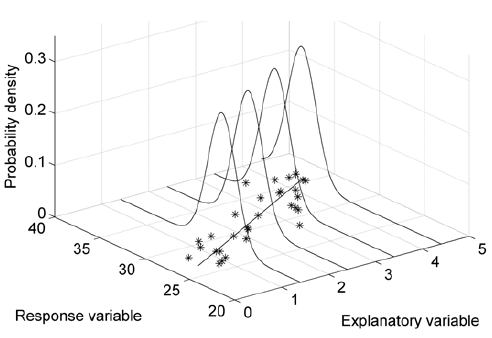
\includegraphics[scale=0.7]{regnorm}
\end{center}
\textcolor{blue}{We assume there is a true underlying line and we observe points about that line.  At every point on the line there is a normal distribution with standard deviation $\sigma$.  The variation about the line is due to unidentified sources (i.e. experimental error).}

\newpage

\textbf{Why use the line instead of just correlation?}%\\~\\~\\~\\~\\~\\
\textcolor{red}{\\~\\Can use line to estimate the mean at a given $x$ and also to find a prediction of a new response for a given $x$.}\\

\Large\textbf{Parameters} to be estimated and make inference on - $\beta_0, \beta_1$ and $\sigma^2$.\large\\
How do we determine these from the data?  Start with $\beta_0$ and $\beta_1$.  Denote the estimates by $\hat\beta_0$ and $\hat\beta_1$.\\~\\
Choice of line determined by minimizing sum of squared residuals:%\\~\\~\\~\\~\\~\\~\\~\\~\\~\\~\\~\\
\textcolor{red}{$$min_{\hat\beta_0,\hat\beta_1}\sum_1^n \left(y_i- (\hat\beta_0 + \hat\beta_1 x_i)\right)^2$$
$$ = \sum_1^n (y_i-\hat{y_i})^2 = \sum_1^n e_i^2 = SS(E)$$
Thus, the resulting $\hat\beta_0$ and $\hat\beta_1$ are called `least squares' estimates.}\\~\\~\\
Calculus can show that $\hat\beta_0$ and $\hat\beta_1$ which minimize the sum of squared residuals $SS(E)$ are given by
$$\hat{\beta}_1=\frac{\sum_{i=1}^{n} (x_i-\bar{x})(Y_i-\bar{Y})}{\sum_{i=1}^{n} (x_i-\bar{x})^2}= \frac{S_{XY}}{S_{XX}} = \frac{s_{XY}}{s_X^2} = \frac{\mbox{sample covariance}}{\mbox{sample variance}} = r_{_{XY}} \frac{s_Y}{s_X}$$
$$\hat{\beta}_0=\bar{Y}-\hat{\beta}_1 \bar{x}$$

\textcolor{blue}{Note: what does $\hat{\beta}_1= r\frac{s_Y}{s_X} $ say about the sign of $r$ and $\hat{\beta}_1$?}\\~\\~\\~\\~\\

The equation using these estimates, $\hat{Y}_i=\hat\beta_0 + \hat\beta_1 x_i$, has many names such as `least squares regression line,' `the fitted line,' `the prediction line,' and `the prediction equation'.\\~\\
$\hat\beta_0$ = sample intercept = %\\
\textcolor{red}{estimated average value of $Y$ when $X = 0$}\\
$$\mu(0)=\beta_0+\beta_10=\beta_0$$
$\hat{\beta}_1$ = sample slope = %\\
\textcolor{red}{estimated change in y (or average y) for a unit change in x (rise/run)}\\

\newpage

Definitions:
\begin{itemize}
\item \textbf{Predicted value} of response $Y$ given $X=x_0$: 
$$ \hat{Y}=\hat\beta_0 + \hat\beta_1 x_0.$$
\item \textbf{Residual} for the $i^{th}$ observation: 
%\\~\\~\\~\\~\\
\textcolor{red}{$$ e_i =y_i-\hat{y}_i = obs - pred$$~\\~\\}
\end{itemize}

The other parameter to estimate is $\sigma^2$.  An {\em unbiased} estimate of $\sigma^2$ for SLR is given by
$$\hat\sigma^2=\frac{SS(E)}{n-2}=MS(E).$$~\\~\\

In lay terms, being unbiased implies that if we did the experiment hundreds of times, finding this estimate for each experiment, then the average of all the MS(E) values $\approx\sigma^2$. \\~\\

For the log(Biodiesel) and Biomass example let`s find our fitted line.  Recall the summary stats on page \pageref{bio}.%\\~\\~\\~\\~\\~\\~\\~\\~\\~\\~\\~\\~\\~\\
\textcolor{red}{
$$\hat\beta_1 = s_{_{XY}}/s_{X}^2 = 3.1485/3.9908^2 =  0.1977$$
$$\hat\beta_0 = 2.4647 - 11.0523*0.1977 = 0.2797$$
$$\hat{y} = 0.2797 + 0.1977x$$}~\\~\\~\\~\\~\\~\\

This line can now be used to make predictions for new $x$ values by simply plugging in the $x$!\\~\\

\newpage

\Large \textbf{How can we make inference (claims about the true values)?}  \large

Our main question is again - do we have a \textit{significant linear relationship?}\\~\\

What value of the slope do we test?
\begin{itemize}
\item If no linear relationship, $Y$ won`t tend to change with $X$ %\\~\\
\textcolor{red}{$$H_0:\beta_1 = 0$$}
\item If a linear relationship, $Y$ will tend to change with $X$ %\\~\\
\textcolor{red}{$$H_A:\beta_1 \neq 0$$}
\end{itemize}

We have a point estimate, $\hat{\beta}_1$, we also need to know about the variability of our estimate.
\begin{eqnarray*}
Var(\hat{\beta}_1)&=&Var\left(\frac{\sum_{i=1}^{n} (x_i-\bar{x})(Y_i-\bar{Y})}{\sum_{i=1}^{n} (x_i-\bar{x})^2}\right)\\
&=&Var\left(\frac{\sum_{i=1}^{n} (x_i-\bar{x})Y_i}{\sum_{i=1}^{n} (x_i-\bar{x})^2}\right)\\
&=&\frac{\sum_{i=1}^{n} (x_i-\bar{x})^2Var(Y_i)}{\left(\sum_{i=1}^{n} (x_i-\bar{x})^2\right)^2} \mbox{    since independent Y's, covariance is 0}\\
&=&\sigma^2\frac{\sum_{i=1}^{n} (x_i-\bar{x})^2}{\left(\sum_{i=1}^{n} (x_i-\bar{x})^2\right)^2}=\frac{\sigma^2}{\sum_{i=1}^{n} (x_i-\bar{x})^2}=\frac{\sigma^2}{S_{xx}}
\end{eqnarray*}
~\\~\\

Under the normal distribution assumption, the RV $\hat\beta_1$ follows normal distribution as it is just a linear combination of normally distributed random variables!%\\~\\~\\~\\
\textcolor{red}{$$\hat{\beta}_1\sim N(\beta,\sigma^2/S_{xx})$$}~\\~\\

What is the standard error of $\hat{\beta}_1$?  As we don't know $\sigma^2$ we will have to estimate it.  What is our estimate for $\sigma^2$?  What is our estimated standard error of $\hat{\beta}_1$?%\\~\\~\\~\\~\\~\\~\\
\textcolor{red}{$$SE(\hat{\beta}_1)=\sqrt{\frac{\sigma^2}{S_{xx}}}$$
$$\hat{\sigma}^2=MS(E)\implies \hat{SE}(\hat{\beta}_1)=\sqrt{\frac{MS(E)}{S_{xx}}}$$}

\newpage

Recall the one-sample Z and the one-sample t-test for $\mu$.  The estimated standard error of $\bar{Y}$ is $\hat{SE}(\bar{Y})=S/\sqrt{n}$.  Our test statistic was
$$Z=\frac{\bar{Y}-\mu_0}{\sigma/\sqrt{n}}\sim N(0,1)~~~~~~~~or~~~~~~~~T=\frac{\bar{Y}-\mu_0}{\hat{SE}(\bar{Y})}=\frac{\bar{Y}-\mu_0}{S/\sqrt{n}}\sim t_{n-1}$$


The same idea applies here!  Any hypothetical slope, like $H_0:\beta_1=\beta_{1,Null}$ may be tested using the $T$-statistic below with $df=n-2$:
$$ T=\frac{\hat\beta_1-\beta_{1,Null}}{\widehat{SE}(\hat\beta_1)}=\frac{\hat\beta_1-\beta_{1,Null}}{\sqrt{MS(E)/S_{xx}}}$$ 
and a $100(1-\alpha)\%$ confidence interval for $\beta_1$ is
$$\hat{\beta}_1 \pm t_{\alpha/2,n-2} \sqrt{\frac{MS(E)}{S_{xx}}}$$

\textcolor{blue}{Note: Tests for the intercept may be performed as well (these will be a special case of testing/intervals for the mean at a given x value). It will depend on the context of the question if testing $\beta_0$=0 makes sense.}\\~\\

\Large\textbf{Locating these tests in the SAS output:}\large\\
\begin{small}
\begin{verbatim}
proc reg data=bioexp ;
model logbiodiesel=biomass/clb;
run;
\end{verbatim}
\end{small}
\begin{flushleft}
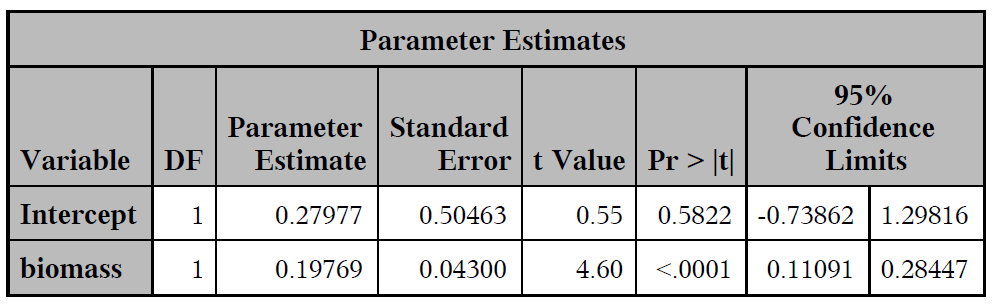
\includegraphics[scale=0.4]{SLRbiodieselparameterestimates}\\
\end{flushleft}

\newpage
\Large \textbf{The ANOVA table for SLR}\large\\
\textit{\textcolor{blue}{An equivalent way to determine if there is a significant linear regression is to use the ANOVA table.}}\\~\\

ANOVA = ANalysis Of VAriance.  What variation are we measuring here?
\begin{flushleft}
\includegraphics[scale=0.4]{slopes}
\end{flushleft}
Which line above gives more evidence of a significant linear relationship?  Why?

\textcolor{red}{The one on the left because the variability around the line is less and yet the variability from the line to the mean is the same as on the right.  \\~\\
This is the idea we use in the ANOVA table.  How much better is the line than just using the mean?  Compare that to how variable the data around the line is (and hence the line itself).}

\newpage

\textbf{Sources of Variability}\\
A measure of the total amount of variability in the response is the sample variance of $Y$.  Consider the numerator, which we call the total sum of squares:
\begin{eqnarray*}
SS(Tot) &= &\sum_{i=1}^n (y_i - \bar{y})^2 \text{   (variability of observations about the mean)}\\
df_{Tot}&=&n-1
\end{eqnarray*}

This variability is partitioned into independent components: \\
Sum of squares due to regression, $SS(R)$
\begin{eqnarray*}
SS(R) & = & \sum_{i=1}^n (\hat{y}_i - \bar{y})^2 \text{     (variability of the fitted line about the mean)}\\
& = & \sum_{i=1}^n (\hat{\beta}_0+\hat{\beta}_1x_i - \hat{\beta}_0-\hat{\beta}_1\bar{x})^2\\
& = & \hat{\beta}_{1}^2S_{xx}\\
df_R & = & 1
\end{eqnarray*}

Sum of squares due to error, $SS(E)$
\begin{eqnarray*}
SS(E) & = & \sum e_i^2 \\
& = & \sum (y_i - \hat{y}_i)^2 \text{    (variability of observations about the fitted line)}\\
df_E & = & n-2
\end{eqnarray*}

~\\~\\
Note: $SS(Tot)=SS(R)+SS(E)$ and $df_{Tot}=df_{R}+df_{E}$  (Recall: DF = Number of independent pieces of data for the sum of squares).\\~\\

\textcolor{red}{In total we have $n$ observations (assumed to be independent).  For $SS(Tot)$ we have to calculate the mean.  Once we have calculated the mean, we only have $n-1$ free observations left.  That is, given any $n-1$ of the $y_i$ values and $\bar{y}$, I can find the remaining $y_i$ value.  Hence, $n-1$ total df.  \\~\\
For $SS(R)$ we have to find $\hat\beta_0$ and $\hat\beta_1$.  However, given one of these two, I can find the other ($\hat{\beta}_0=\bar{y}-\hat{\beta}_1\bar{x}$).  Therefore, there are $2-1=1$ df for regression.\\~\\
This leaves $n-2$ df for error.}

\newpage

\cu{The ANOVA table from simple linear regression}
\begin{tabular}{|c|c|c|c|c|} \hline
Source &  df & Sum of squares &Mean Square & F-Ratio \\ \hline
Regression & 1& $SS(R)$  & $MS(R)$ & $MS(R)/MS(E)\sim^{H_0} F_{1,n-2}$ \\
Error & $n-2$ & $SS(E)$  & $MS(E)$ &  \\
Total & $n-1$ & $SS(Tot)$  & &  \\ \hline
\end{tabular}

~\\The mean squares represent standardized measures of variation due to the different sources and are given by $SS(source)/df source$.  Ratios of mean squares often follow an $F$-distribution and are appropriate for testing different hypotheses of interest.\\~\\
In this case, to test \\~\\
$ H_0: \beta_1 = 0 \mbox{  vs  } H_1:\beta_1 \neq 0$\\~\\
The test statistic is 
$$F = MS(R)/MS(E) \stackrel{H_0}{\sim} F(1,n-2).$$~\\
The rejection region is 
$$\left\{F_{obs}:F_{obs}>F_{\alpha,1,n-2}\right\}$$~\\
The p-value is
$$P(F_{1,n-2}>F_{obs})$$~\\

This $F$ test is equivalent to the $t$ test we already looked at.  The relationship is that $(t_{df})^2=F_{1,df}$.  \\~\\
Large values of $F$ give evidence that the line is useful.  Values near 1 imply that using the mean of the response is just as useful as the line.\\~\\

\newpage

\textbf{How to get the ANOVA table in SAS?}\\
For our Biodiesel and Biomass example we can get our output from SAS using the following commands:
\begin{small}
\begin{verbatim}
proc reg data=bioexp ;
model logbiodiesel=biomass/clb;
run;
\end{verbatim}
\end{small}
~\\
\begin{flushleft}
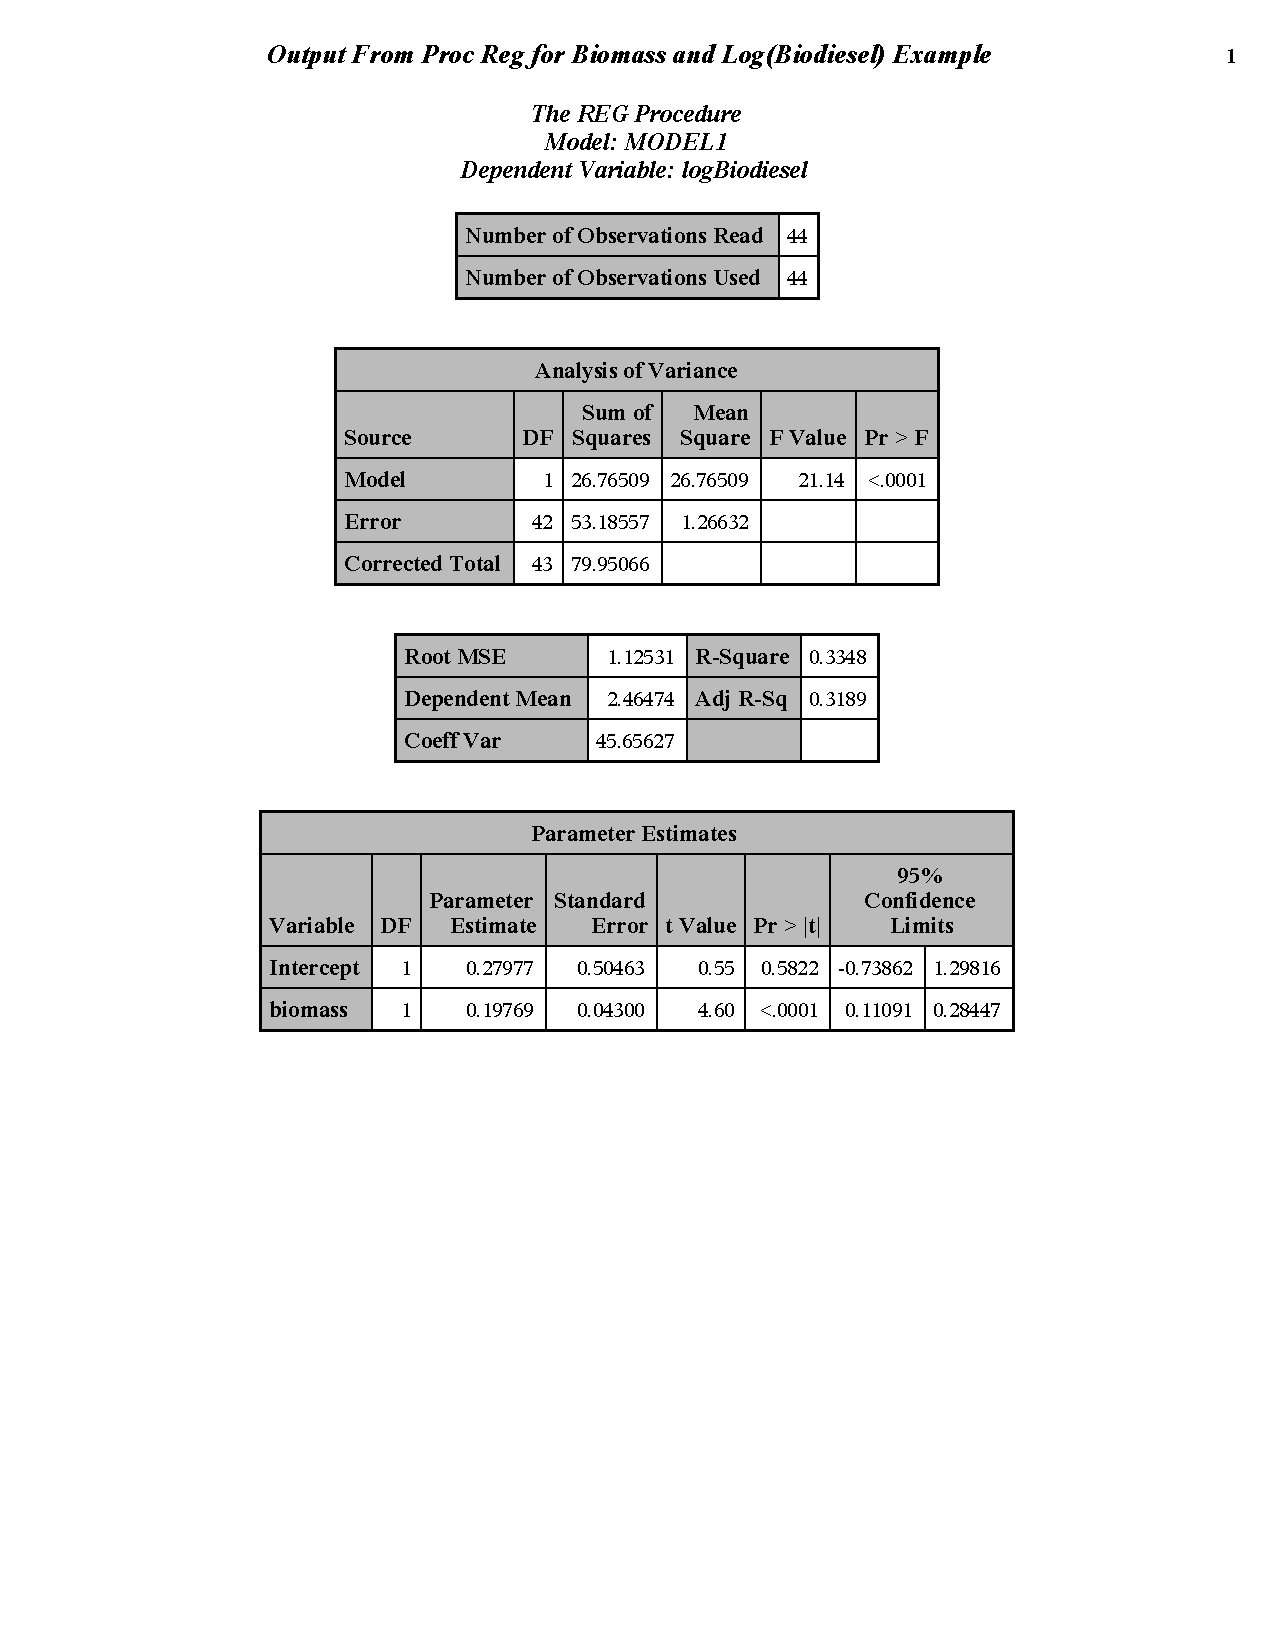
\includegraphics[scale=0.8,trim= 10mm 105mm 10mm 10mm]{slrbiodiesel}\\
\end{flushleft}
~\\


\newpage

\Large \textbf{Other Inferential Objectives}\large\\
\textcolor{blue}{One reason to consider SLR instead of correlation analysis is that we can now make predictions for the response.\\~\\
Let`s consider a prediction made from this model.  If the experiment were run again, would we get the same fitted line? The same predicted mean value?} \\~\\~\\~\\~\\~\\

The predicted mean is itself a RV and so we can find CI for that mean!  We can also create a `Prediction Interval' (PI) for a new $x$ value as well.\\~\\

\textbf{Confidence interval for $\mu(x_0) = E(Y|X=x_0)$} ($x_0$ a value of interest)\\
The point estimate for $\mu(x_0)$ is $\hat\beta_0+\hat\beta_1x_0$.  We need to know about the variability of this estimate and we can again use the t-distribution for inference.
\begin{eqnarray*}
\Var(\hat\beta_0+\hat\beta_1 x_0)
& = & \Var(\bar{Y}-\bar{x}\hat{\beta}_1+\hat{\beta}_1 x_0)\\
& = & \Var(\bar{Y}-\hat{\beta}_1(\bar{x}-x_0))\\
& = & \sigma^2/n + \sigma^2\frac{(x_0-\bar{x})^2}{S_{xx}}~~~~~~Cov(\bar{Y},\hat{\beta}_1)=0\\
& = & \sigma^2\left(\frac{1}{n} + \frac{(x_0-\bar{x})^2}{S_{xx}}\right)
\end{eqnarray*}
Again, we estimate $\sigma^2$, yielding a CI for $\mu(x_0)$ of
$$\hat\beta_0 +\hat\beta_1 x_0 \pm t_{n-2,\alpha/2} \sqrt{MS(E)\left(\frac{1}{n}+\frac{(x_0-\bar{x})^2}{S_{xx}}\right)} $$
**Note: We are attempting to capture \textbf{the true mean of all responses with an x-value of $x_0$}.\\~\\

\newpage

\textbf{Prediction interval for a new observation $x_0$}\\
The point estimate for at $x_0$ is still $\hat{Y}(x_0)=\hat\beta_0+\hat\beta_1x_0$.  However, the variability will change.
\begin{eqnarray*}
\Var(\hat\beta_0+\hat\beta_1 x_0+E_{new}|X=x_0)
& = & \sigma^2\left(\frac{1}{n} + \frac{(x_0-\bar{x})^2}{S_{xx}}\right)+\sigma^2~~~~~\mbox{As }E_{new}\mbox{ is independent of past Y's}\\
& = & \sigma^2\left(1+\frac{1}{n} + \frac{(x_0-\bar{x})^2}{S_{xx}}\right)
\end{eqnarray*}

Thus we can form a PI using
$$\hat\beta_0 +\hat\beta_1 x_0 \pm t_{n-2,\alpha/2} \sqrt{MS(E)\left(1+\frac{1}{n}+\frac{(x_0-\bar{x})^2}{S_{xx}}\right)}. $$
**Note: In this interval we are attempting to capture \textbf{the next $Y$ value that takes on $x_0$}.  As this is a much more difficult task, PI`s are wider than CI`s.  \\~\\~\\

For a SLR model, Proc Reg in SAS will also produce a very nice plot that includes \textit{pointwise} confidence and prediction bands at all observed x's. \\
Notice that the bands get wider the further $x_0$ is from $\bar{x}$.  Why? \textcolor{red}{Most info at $\bar{x}$}

\begin{flushleft}
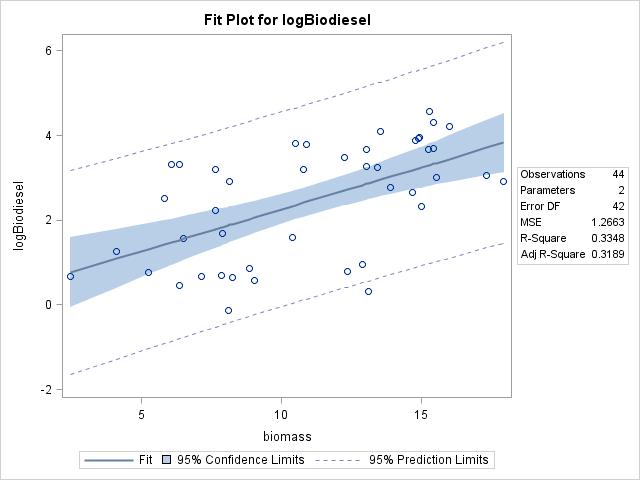
\includegraphics[scale=0.6]{biofitpred}
\end{flushleft}

\textcolor{blue}{A note of caution: We should only use our line to predict for $X$ values within the observed range (interpolating).  Extrapolating (predicting for an $X$ outside the range of observed X's) is dangerous as we don't know if the linear pattern exists outside the observed X's.\\~\\
Example: Consider measuring the heights of 4-16 year old people.  There is likely to be a strong positive correlation between height and age.  Consider fitting a line and using it to predict height for a 40 year old!}


Using $\alpha=0.05$, ($t_{n-2,\alpha/2}=t_{42,0.025}=2.0181$) (Use, $SS(R)=\hat{\beta}_1^2S_{xx}\implies S_{xx}=26.76509/0.19769^2=684.8561$)
\begin{enumerate}
\item Find the CI for slope by hand.
\item Form a CI for the mean log of biodiesel when biomass is 12.
\item Form a PI for a future log biodiesel measurement for a biomass of 12.\\
\textcolor{blue}{Note: In lab you will see an easy way to find the CI and PI intervals at a given $x$ using SAS and the `missing y' trick!}
\end{enumerate}

\begin{enumerate}
\item \textcolor{red}{The CI for the slope is 
$$\hat{\beta}_1 \pm t_{n-2,\alpha/2} \sqrt{\frac{MS[E]}{S_{xx}}}$$
From the output we have $\hat{\beta}_1=0.1977$ and $MS(E)=1.2663$.  
Thus, we are 95\% confident that the true slope between biomass and log(biodiesel) ($\beta_1$) is in the interval
$$0.19769 \pm 2.0181\sqrt{1.26632/684.8561}=(0.1109, 0.2845).$$
\item The CI for a mean response is given by 
$$\hat\beta_0 +\hat\beta_1 x_0 \pm t_{n-2,\alpha/2} \sqrt{MS(E)\left(\frac{1}{n}+\frac{(x_0-\bar{x})^2}{S_{xx}}\right)} $$  
We already have most of the things we need from part (1).  Our prediction for a biomass of 12 is 
$$0.2798+0.1977*12=2.6522,$$
the sample size is $n=44$, and we can find $\bar{x}$= 11.0523 from the correlation output on page \pageref{corrbio}.  \\
Thus, we are 95\% confident that the true mean log biodiesel for a plant with a biomass of 12 is in the interval
$$2.6522 \pm 2.0181\sqrt{1.2663(1/44+(12-11.0523)^2/684.787)}=(2.3001,3.0043).$$
\item The PI for a future response is given by 
$$\hat\beta_0 +\hat\beta_1 x_0 \pm t_{n-2,\alpha/2} \sqrt{MS(E)\left(1+\frac{1}{n}+\frac{(x_0-\bar{x})^2}{S_{xx}}\right)} $$
Thus, we are 95\% confident that a future log biodiesel measurement for a plant with a biomass of 12 is in the interval
$$2.6522 \pm 2.0181\sqrt{1.2663(1+1/44+(12-11.0523)^2/684.787)}=(0.3541,4.9503).$$
\textbf{Note: To make these intervals more meaningful we may want to exponentiate the end points of the intervals to put them on the scale of the original data.}}
\end{enumerate}

\newpage

\Large\textbf{$R^2$ - the coefficient of determination}\large\\

Ideally, our model will account for most of the variation in the response.\\~\\

To look at this, we create the ratio of $SS(R)$ to $SS(TOT)$ 
$$R^2=\frac{SS(R)}{SS(Tot)}$$
If $R^2$ is close to 1, then the model fits the data very well.\\~\\

$R^2$ is also called the {\em coefficient of determination}.  \\~\\

For the log(biodiesel) and biomass example $r^2=26.76509/79.95066=0.5786^2= 0.335$.  In simple linear regression, 'r-square' is in fact equal to $R_{_{XY}}^2$.  (This isn't the case in multiple regression or other models.)\\~\\

The interpretation of $R^2$ usually goes as follows:\\~\\

\textcolor{red}{33.5\% of variation in log(biodiesel) can be explained by the linear association between log(biodiesel) and biomass.}

\newpage



\Large \textbf{Checking Model Assumptions in SLR}\large\\

\textcolor{blue}{Once we have fit our model and looked at our test we need to consider the validity of our assumptions for the SLR model.  Namely, that there is a true linear relationship and our errors are iid $N(0,\sigma^2)$ for all x.}\\~\\

\textbf{Checking assumptions}
\begin{enumerate}
\item Inspect a scatter plot to determine if the linear relationship we are assuming in our model is appropriate.
\item Assumption of $iid~N(0,\sigma^2)$ errors:
\begin{itemize}
\item Independence - There is not a check for independence of errors,  we simply need to consider whether or not our EUs can be considered independent. (Although, if the responses are time dependent we could plot them vs time.)
\item Constant variance - A residuals vs fitted (predicted) values plot or a residual vs independent variable plot are tools for detecting heteroskedasticity (non-constant variance).    We hope to see a random scattering of points with no clear trends.
\begin{center}
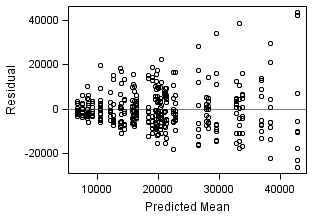
\includegraphics[scale=0.8]{hetero}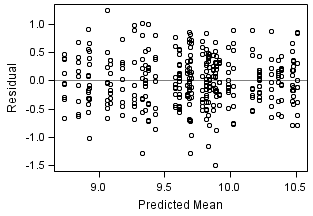
\includegraphics[scale=0.9]{homo}
\end{center}
\item Normality of errors - A quantile-quantile plot (or qq-plot for short) can be inspected to see if normality is reasonable.  We hope to see a straight line.\\
\begin{center}
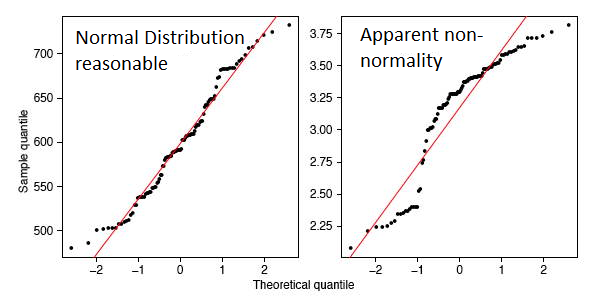
\includegraphics[scale=0.45]{qq}
\end{center}
\end{itemize}
\end{enumerate}

\textbf{More on qq-plots}\\
The $p^{th}$ quantile (or percentile) of a distribution is the value that has $p$ \% of the distribution below it.\\

If we have $n$ observations we can get observed quantiles for the data and create the qq-plot.
\begin{enumerate}
\item Sort the data from smallest to largest.
\item The $i^{th}$ ordered data point is the observed $\frac{(i-0.5)}{n}$ quantile
(There are other formulas used for this as well.)
\item Find the corresponding theoretical quantiles.
\item Plot the pairs of points.
\end{enumerate}

The idea of a qq-plot is to compare the observed quantiles to theoretical ones from a particular distribution (often the normal).  If the distribution is a good fit, the observed and theoretical quantiles will be spread out in the same manner and should roughly fall in a line.\\

Ex: Consider the data set consisting of the following (ordered) observations: 
$$0.44,	1.67,	1.88,	2.45,	3.01$$
Is the normal distribution a good fit for this data?\\

\begin{tabular}{cc|c|c}
Ordered Observed & i & Observed Quantile (i-0.5)/n & Corresponding Normal Quantile\\
\hline
0.44 & 1 & 0.1 & -1.28\\
1.67 & 2 & 0.3 & -0.52\\
1.88 & 3 & 0.5 & 0.00\\
2.45 & 4 & 0.7 & 0.52\\
3.01 & 5 & 0.9 & 1.28\\
 & & `y-values' & 'x-values'
\end{tabular}

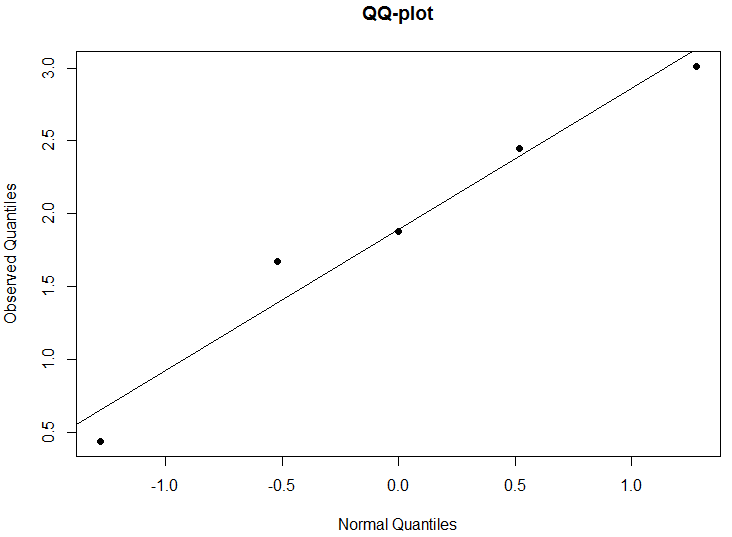
\includegraphics[scale=0.45]{qqplot}

\newpage

We can inspect the diagnostic plots that SAS produces when the reg procedure is used:
\begin{center}
\includegraphics[scale=0.65,page=2,trim= 10mm 70mm 10mm 10mm]{slrbiodiesel}\\
\includegraphics[scale=0.4,page=3,trim= 10mm 100mm 10mm 10mm]{slrbiodiesel}\\
\end{center}

\newpage

\textbf{An exercise: Match up letters a,b,c,d with the model violation - Heteroskedasticity, Nonlinearity, Nonnormality, Model fits}
\begin{center}
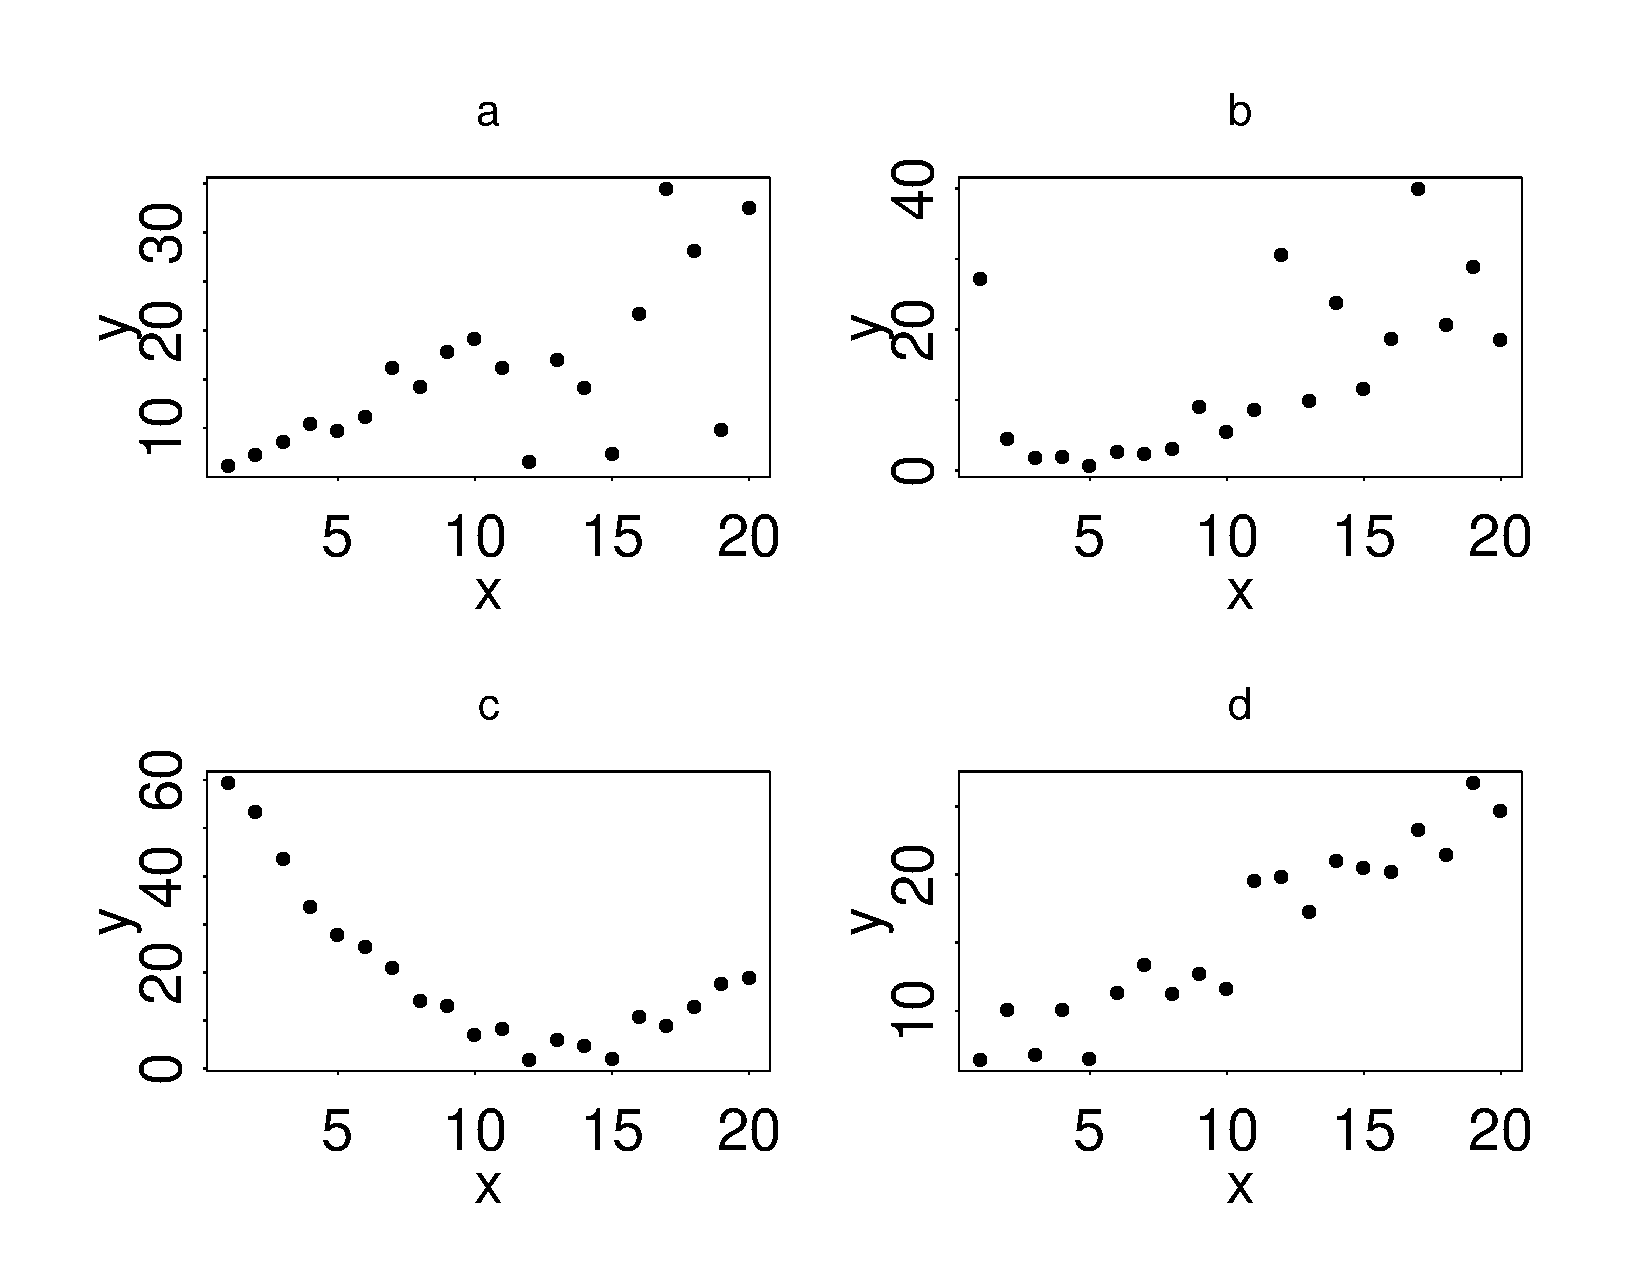
\includegraphics[height=2.5in,width=3in]{ybyx_handout.pdf}
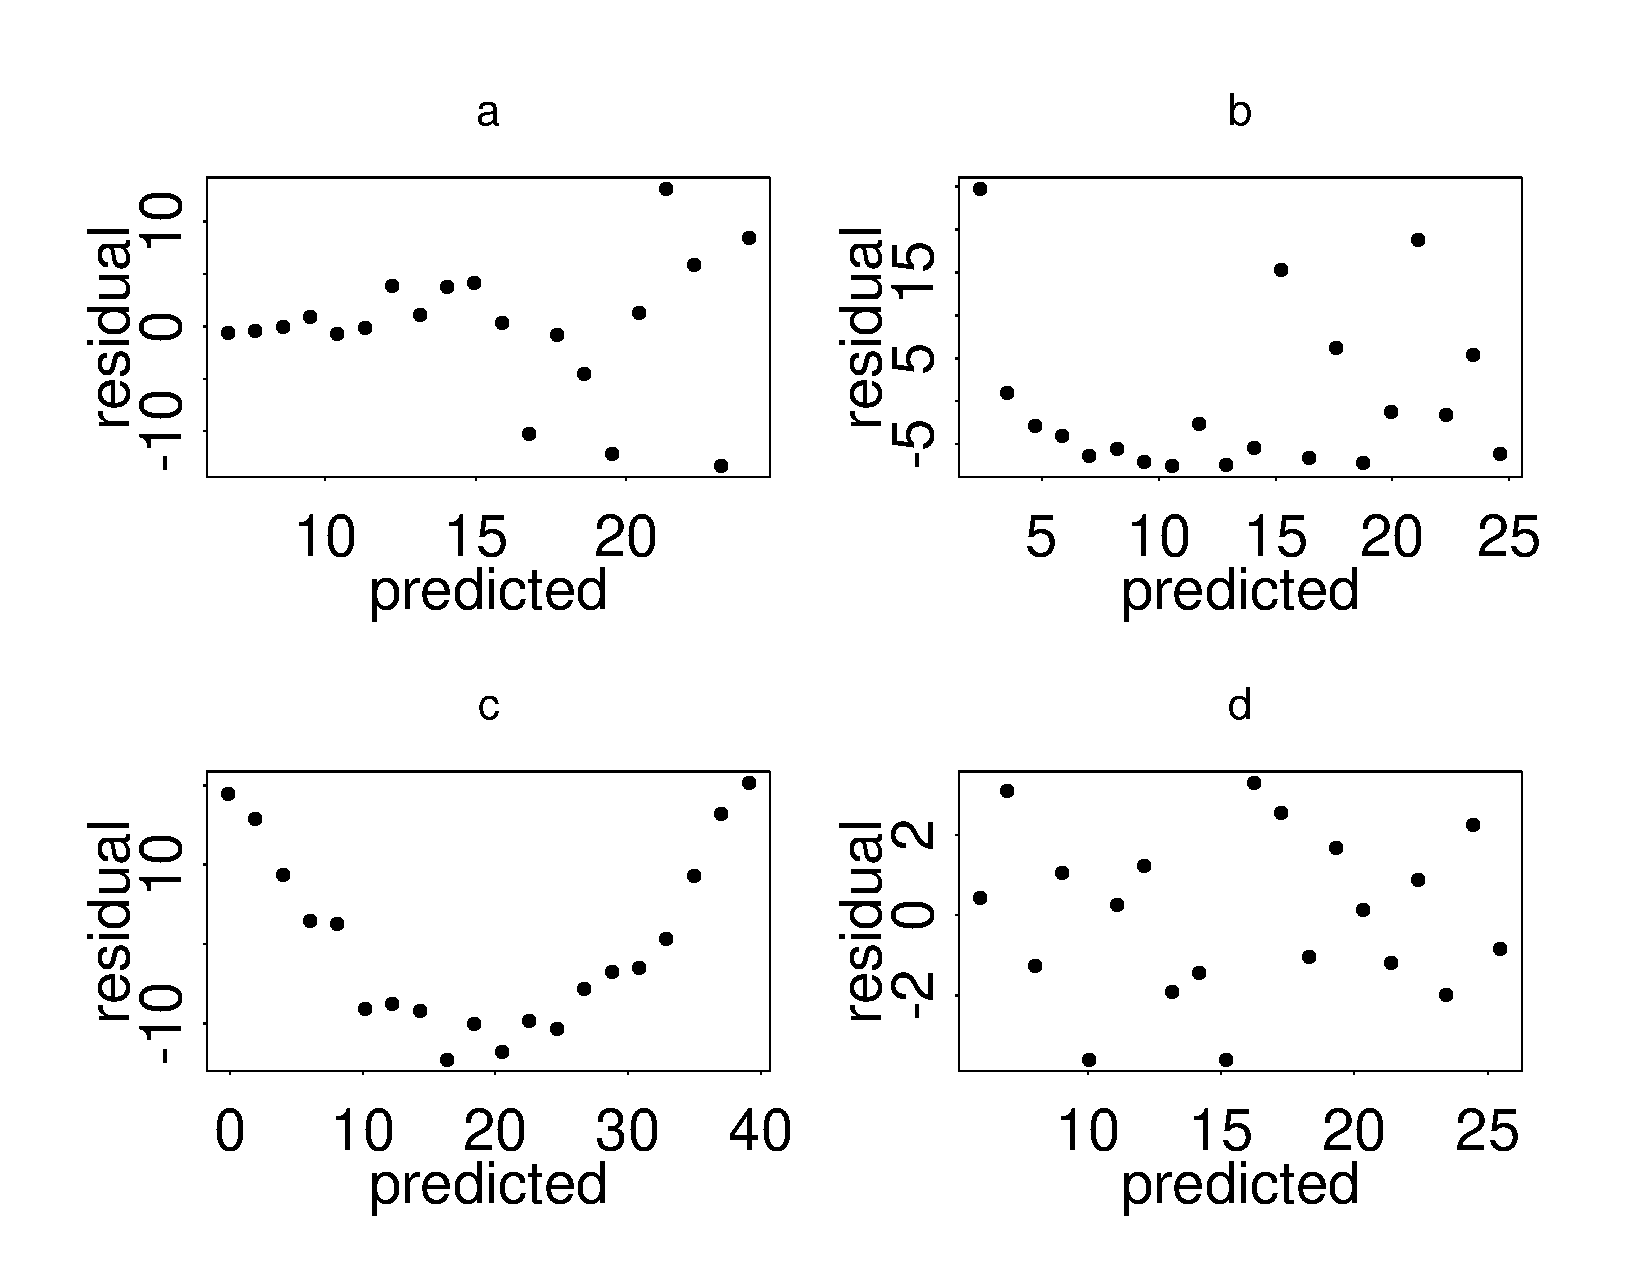
\includegraphics[height=2.5in,width=3in]{resbypred_handout.pdf}
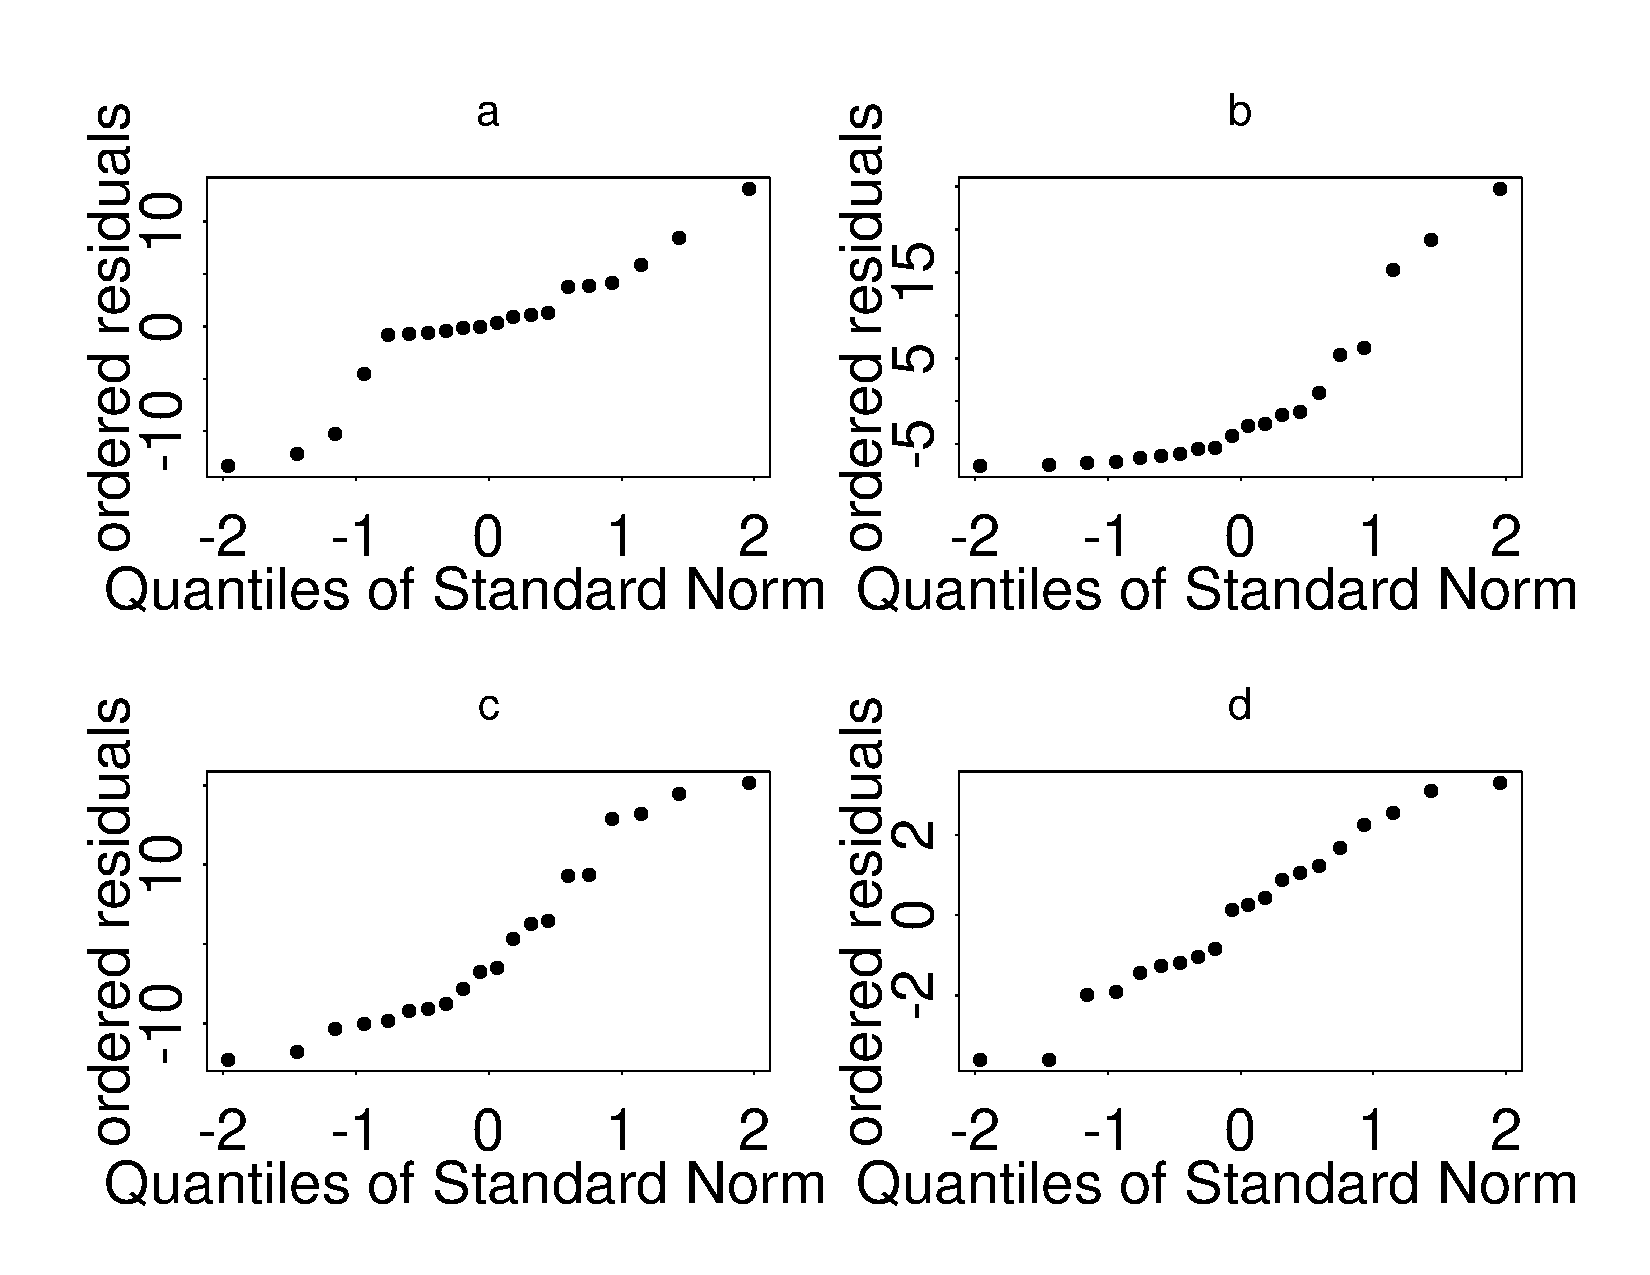
\includegraphics[height=2.5in,width=3in]{qqnorm_handout.pdf}
\end{center}

\textcolor{red}{a=Heteroskedasticity, b = Nonnormality, c = nonlinearity, d=model fits}\\

\textcolor{blue}{\textbf{What to do when assumptions are violated?} - Transformations of the data can often resolve fit issues.  (For instance, we have been working with log(biodiesel) for just that reason.)  You will take up transformations of data in lab!}\\~\\~\\


\textit{\textcolor{blue}{This wraps up the discussion of Correlation and SLR.  We will now consider expanding the ideas used in SLR to the case when we have multiple quantitative explanatory variables.  Then things get really exciting when we use these ideas to then also include categorical explanatory variables in what are called general linear models (GLMs)}}





